% Copyright 2004 by Till Tantau <tantau@users.sourceforge.net>.
%
% In principle, this file can be redistributed and/or modified under
% the terms of the GNU Public License, version 2.
%
% However, this file is supposed to be a template to be modified
% for your own needs. For this reason, if you use this file as a
% template and not specifically distribute it as part of a another
% package/program, I grant the extra permission to freely copy and
% modify this file as you see fit and even to delete this copyright
% notice.

\documentclass[xcolor=dvipsnames, 14pt]{beamer}
\usepackage{listings}
\usepackage{fancyvrb}
%\usepackage[usenames,dvipsnames]{xcolor}
%\usepackage{graphicx}
%\usepackage{textpos}
% There are many different themes available for Beamer. A comprehensive
% list with examples is given here:
% http://deic.uab.es/~iblanes/beamer_gallery/index_by_theme.html
% You can uncomment the themes below if you would like to use a different
% one:
%\usetheme{AnnArbor}
%\usetheme{Antibes}
%\usetheme{Bergen}
%\usetheme{Berkelesdy}
%\usetheme{Berlin}
%\usetheme{Boadilla}
%\usetheme{boxes}
%\usetheme{CambridgeUS}
%\usetheme{Copenhagen}
%\usetheme{Darmstadt}
%\usetheme{default}
%\usetheme{Frankfurt}
%\usetheme{Goettingen}
%\usetheme{Hannover}
%\usetheme{Ilmenau}
%\usetheme{JuanLesPins}
%\usetheme{Luebeck}
\usetheme{Madrid}
%\usetheme{Malmoe}
%\usetheme{Marburg}
%\usetheme{Montpellier}
%\usetheme{PaloAlto}
%\usetheme{Pittsburgh}
%\usetheme{Rochester}
%\usetheme{Singapore}
%\usetheme{Szeged}
%\usetheme{Warsaw}
\addtobeamertemplate{title page}{ 
\includegraphics[scale=0.1]{img/IST_A_RGB_POS3.png} }{} %por a imagem no canto superior esquerdo.

\title{Refactoring for Dynamic Languages}

% A subtitle is optional and this may be deleted
%\subtitle{Optional Subtitle}
%\begin{textblock*}{2cm}(1cm,-7.5cm)
%  
\includegraphics[width=2cm]{img/IST_A_RGB_POS.png}% use the \includegraphics command here
%\end{textblock*}


\author{Rafael Reia }
% - Give the names in the same order as the appear in the paper.
% - Use the \inst{?} command only if the authors have different
%   affiliation.


\institute[Universidade de Lisboa] % (optional, but mostly needed)
{

  Instituto Superior T\'ecnico\\
  Universidade de Lisboa \\
  %
\includegraphics[scale=0.1]{img/IST_A_RGB_POS.png}
  }
% - Use the \inst command only if there are several affiliations.
% - Keep it simple, no one is interested in your street address.

\date{26th Jun, 2015}
% - Either use conference name or its abbreviation.
% - Not really informative to the audience, more for people (including
%   yourself) who are reading the slides online

\subject{Refactoring for Dynamic Languages}
% This is only inserted into the PDF information catalog. Can be left
% out.

% If you have a file called "university-logo-filename.xxx", where xxx
% is a graphic format that can be processed by latex or pdflatex,
% resp., then you can add a logo as follows:

% \pgfdeclareimage[height=0.5cm]{university-logo}{university-logo-filename}
% \logo{\pgfuseimage{university-logo}}

% Delete this, if you do not want the table of contents to pop up at
% the beginning of each subsection:
\AtBeginSection[]
{
  \begin{frame}<beamer>{Outline}
    \tableofcontents[currentsection,currentsubsection]
  \end{frame}
}

% Let's get started
\begin{document}
\defverbatim[colored]\mycode{%
\begin{lstlisting}[frame=single, label={lst:Fibonacci}, emph={define, let, if, cons, for, displayln, in-list},  emphstyle={\bf\color{blue}}] %\color{blue}

(define (fibs n)
  (let ((fibs
         (let loop ((previous 0)
                    (current 1)
                    (index 0))
           (if (= index n)
               (list)
               (cons current
                     (loop current
                           (+ previous current)
                           (+ index 1)))))))
    (for ((fib (in-list fibs)))
      (displayln fib))))
\end{lstlisting}
}

\defverbatim[colored]\mycodeE{%
\begin{lstlisting}[frame=single, label={lst:Fibonacci}, emph={define, let, if, cons, for, displayln, in-list},  emphstyle={\bf\color{blue}}] %\color{blue}

(define (print-list fibs)
  (for ((fib (in-list fibs)))
      (displayln fib)))
(define (fibs n)
  (let ((fibs
         (let loop ((previous 0)
                    (current 1)
                    (index 0))
           (if (= index n)
               (list)
               (cons current
                     (loop current
                           (+ previous current)
                           (+ index 1)))))))
    (print-list fibs)))

\end{lstlisting}
}
\defverbatim[colored]\mycodeEx{%
\begin{lstlisting}[frame=single, label={lst:Fibonacci}, emph={define, let, if, cons, for, displayln, in-list},  emphstyle={\bf\color{blue}}] %\color{blue}

(define (print-list fibs)
  (for ((fib (in-list fibs)))
      (displayln fib)))
(define (compute-fibonacci n)
  (let loop ((previous 0)
                    (current 1)
                    (index 0))
           (if (= index n)
               (list)
               (cons current
                     (loop current
                           (+ previous current)
                           (+ index 1))))))
(define (fibs n)
  (let ((fibs
         (compute-fibonacci n)))
    (print-list fibs)))

\end{lstlisting}
}


\begin{frame}
  \titlepage
\end{frame}

\begin{frame}{Outline}
  \tableofcontents[] % subsectionsonly , pausesections
  % You might wish to add the option [pausesections]
\end{frame}

% Section and subsections will appear in the presentation overview
% and table of contents.
\section{Introduction}
\subsection{Motivation}

\begin{frame}{Motivation}
\begin{figure}[htbp]
  \centering
  
\includegraphics[width=0.95\textwidth]{img/softwareEvolution.png}
  %\caption{Before the Rename}
  \label{fig:SE}
\end{figure}
\end{frame}
\begin{frame}[fragile]{Motivation}
%Fibonacci example
\begin{Verbatim}[fontsize=\footnotesize]
(define (fibs n)
  (let ((fibs
         (let loop ((previous 0)
                    (current 1)
                    (index 0))
           (if (= index n)
               (list)
               (cons current
                     (loop current
                           (+ previous current)
                           (+ index 1)))))))
    (for ((fib (in-list fibs)))
      (displayln fib))))
\end{Verbatim}
\end{frame}

\fvset{gobble=2}
\begin{frame}[fragile]{Motivation}
%Fibonacci example
\fvset{gobble=2}
\begin{Verbatim}[fontsize=\footnotesize]
  (define (fibs n)
    (let ((fibs
           (let loop ((previous 0)
                      (current 1)
                      (index 0))
             (if (= index n)
                 (list)
                 (cons current
                       (loop current
                             (+ previous current)
                             (+ index 1)))))))
\end{Verbatim}
% framesep=0mm
\begin{Verbatim}[frame=single, rulecolor=\color{red}, fontsize=\footnotesize]
      (for ((fib (in-list fibs)))
        (displayln fib))))
\end{Verbatim}
\end{frame}
\begin{frame}[fragile]{Motivation}
%Fibonacci example

\fvset{globble=3}
\begin{Verbatim}[frame=single, rulecolor=\color{red}, fontsize=\footnotesize]
  (define (print-list fibs)
    (for ((fib (in-list fibs)))
      (displayln fib)))
\end{Verbatim}
\begin{Verbatim}[fontsize=\footnotesize]
  (define (fibs n)
    (let ((fibs
           (let loop ((previous 0)
                      (current 1)
                      (index 0))
             (if (= index n)
                 (list)
                 (cons current
                       (loop current
                             (+ previous current)
                             (+ index 1)))))))
\end{Verbatim}
\begin{Verbatim}[frame=single, rulecolor=\color{red}, fontsize=\footnotesize]
      (print-list fibs)))
\end{Verbatim}
\end{frame}
\begin{frame}[fragile]{Motivation}
%Fibonacci example
\fvset{globble=3}
\begin{Verbatim}[fontsize=\footnotesize]
  (define (print-list fibs)
    (for ((fib (in-list fibs)))
      (displayln fib)))

  (define (fibs n)
    (let ((fibs
    \end{Verbatim}
\begin{Verbatim}[frame=single, rulecolor=\color{red},fontsize=\footnotesize]
           (let loop ((previous 0)
                      (current 1)
                      (index 0))
             (if (= index n)
                 (list)
                 (cons current
                       (loop current
                             (+ previous current)
                             (+ index 1)))))))
\end{Verbatim}
\begin{Verbatim}[fontsize=\footnotesize]
      (print-list fibs)))
\end{Verbatim}
\end{frame}


\begin{frame}[fragile]{Motivation}
%Fibonacci example

\fvset{globble=4}
\begin{Verbatim}[frame=single, rulecolor=\color{red},fontsize=\footnotesize]
  (define (compute-fibonacci n)
    (let loop ((previous 0)
               (current 1)
               (index 0))
      (if (= index n)
          (list)
          (cons current
                (loop current
                      (+ previous current)
                      (+ index 1))))))
\end{Verbatim}
\begin{Verbatim}[fontsize=\scriptsize]
  (define (print-list fibs)
    (for ((fib (in-list fibs)))
      (displayln fib)))

  (define (fibs n)
    (let ((fibs
\end{Verbatim}
\begin{Verbatim}[frame=single, rulecolor=\color{red},fontsize=\footnotesize]
           (compute-fibonacci n)))
\end{Verbatim}
\begin{Verbatim}[fontsize=\scriptsize]
      (print-list fibs)))
\end{Verbatim}
\end{frame}

\begin{frame}{Copy Paste - What can go wrong}
\begin{figure}[htbp]
  \centering
  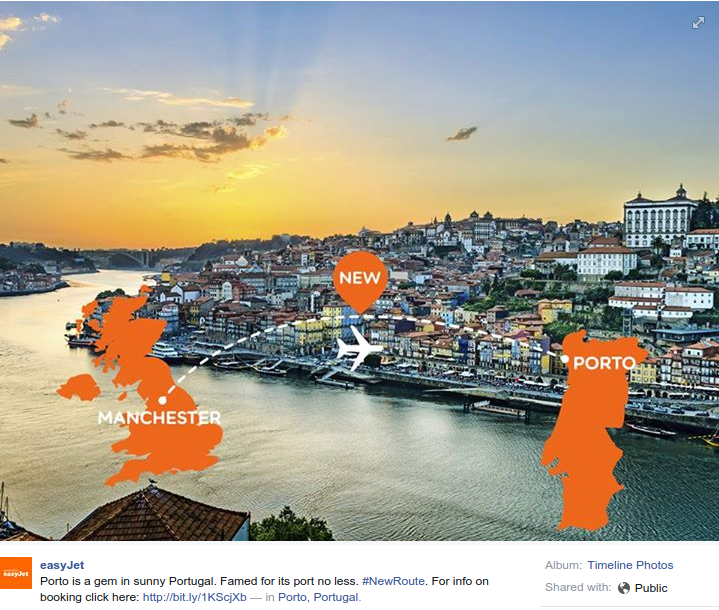
\includegraphics[width=0.7\textwidth]{img/WhatCanGoWrongWithCopyPaste1.png}
  %\caption{Before the Rename}
  \label{fig:CopyPaste}
\end{figure}
\end{frame}
\begin{frame}{Copy Paste - What can go wrong}
\begin{figure}[htbp]
  \centering
  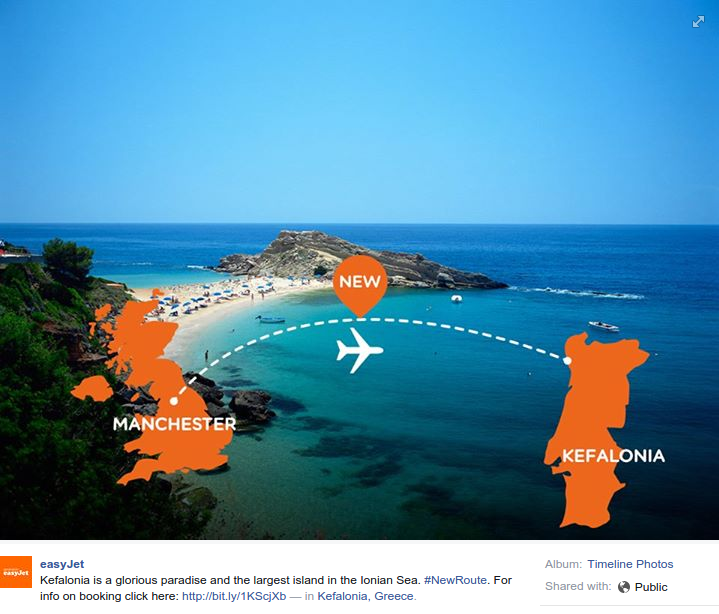
\includegraphics[width=0.7\textwidth]{img/WhatCanGoWrongWithCopyPaste.png}
  %\caption{Before the Rename}
  \label{fig:CopyPaste-error}
\end{figure}
\end{frame}
\begin{frame}{Motivation}
  \begin{itemize}
  \setlength\itemsep{2em}
  \item {
    Lack of Refactoring tools for Dynamic Languages
  }
  \item {
    Lack of Refactoring tools adequate to beginners
  }
  \end{itemize}
\end{frame}
\subsection{Objectives}

\begin{frame}{Objectives}%{Optional Subtitle}
  \begin{itemize}
  \setlength\itemsep{2em}
  \item {
    Correct
  }
  \item {
    Useful
  }
  \item {
    Simple to use
  }
  \end{itemize}
\end{frame}

\subsection{Definitions}
\begin{frame}{Refactoring Correctness}
\begin{itemize}
\setlength\itemsep{2em}
\item Formal Approach
\item Informal Approach
\end{itemize}
\end{frame}
\begin{frame}{Refactoring tools - Classification}
  \begin{itemize}
  \setlength\itemsep{2em}
  \item {
    Manual
  }
  \item {
    Semi-Automatic
  }
  \item {
    Fully-Automatic
  }
  \end{itemize}
\end{frame}
\section{Related Work}
% You can reveal the parts of a slide one at a time
% with the \pause command:
%\begin{frame}{How we Refactor}

%\end{frame}
\begin{frame}{How we Refactor}
  \begin{itemize}
  \setlength\itemsep{2em}
  \item {
  Done continuously
  }
  \item {
    Differs among users
  }
  \item {
    Refactoring tools are underused
  }
  \end{itemize}
\end{frame}
\begin{frame}{Scheme}
    \begin{figure}[htbp]
      \centering
      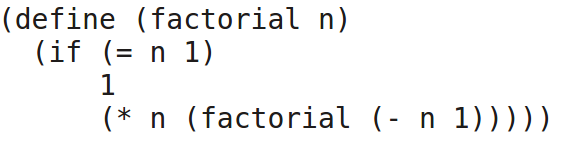
\includegraphics[width=0.75\textwidth]{img/SchemeCode2.png}
      %\caption{Before the Rename}
      \label{fig:Scheme}
    \end{figure}
\end{frame}

\begin{frame}{SmallTalk}
  \begin{figure}[htbp]
    \centering
    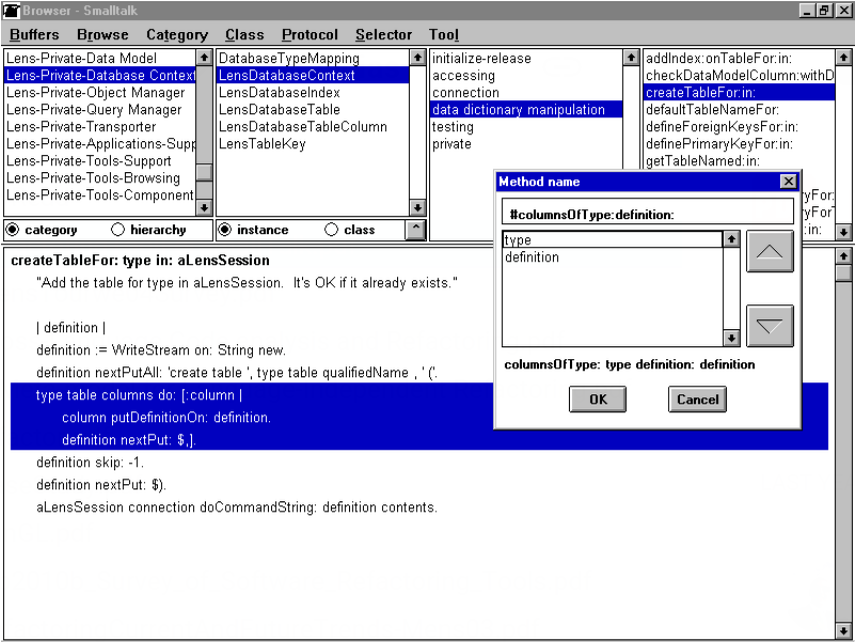
\includegraphics[width=0.7\textwidth]{img/smalltalk.png}
    %\caption{Before the Rename}
    \label{fig:Smalltalk}
  \end{figure}
\end{frame}

\begin{frame}{JavaScript}
  \begin{figure}[htbp]
    \centering
    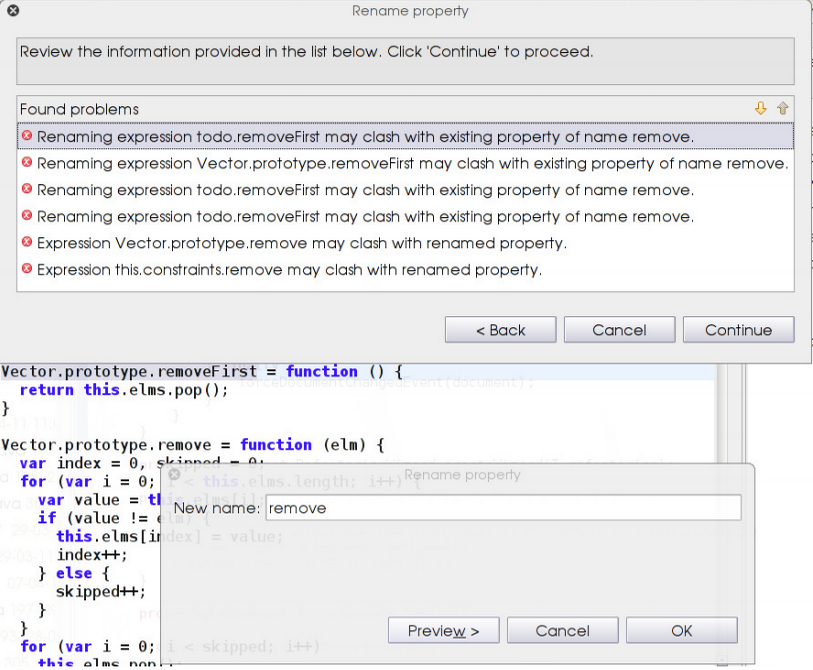
\includegraphics[width=0.7\textwidth]{img/Javascript.png}
    %\caption{Before the Rename}
    \label{fig:JavaScript}
  \end{figure}
\end{frame}


%\begin{frame}{Python}
%  \begin{figure}[htbp]
%    \centering
%    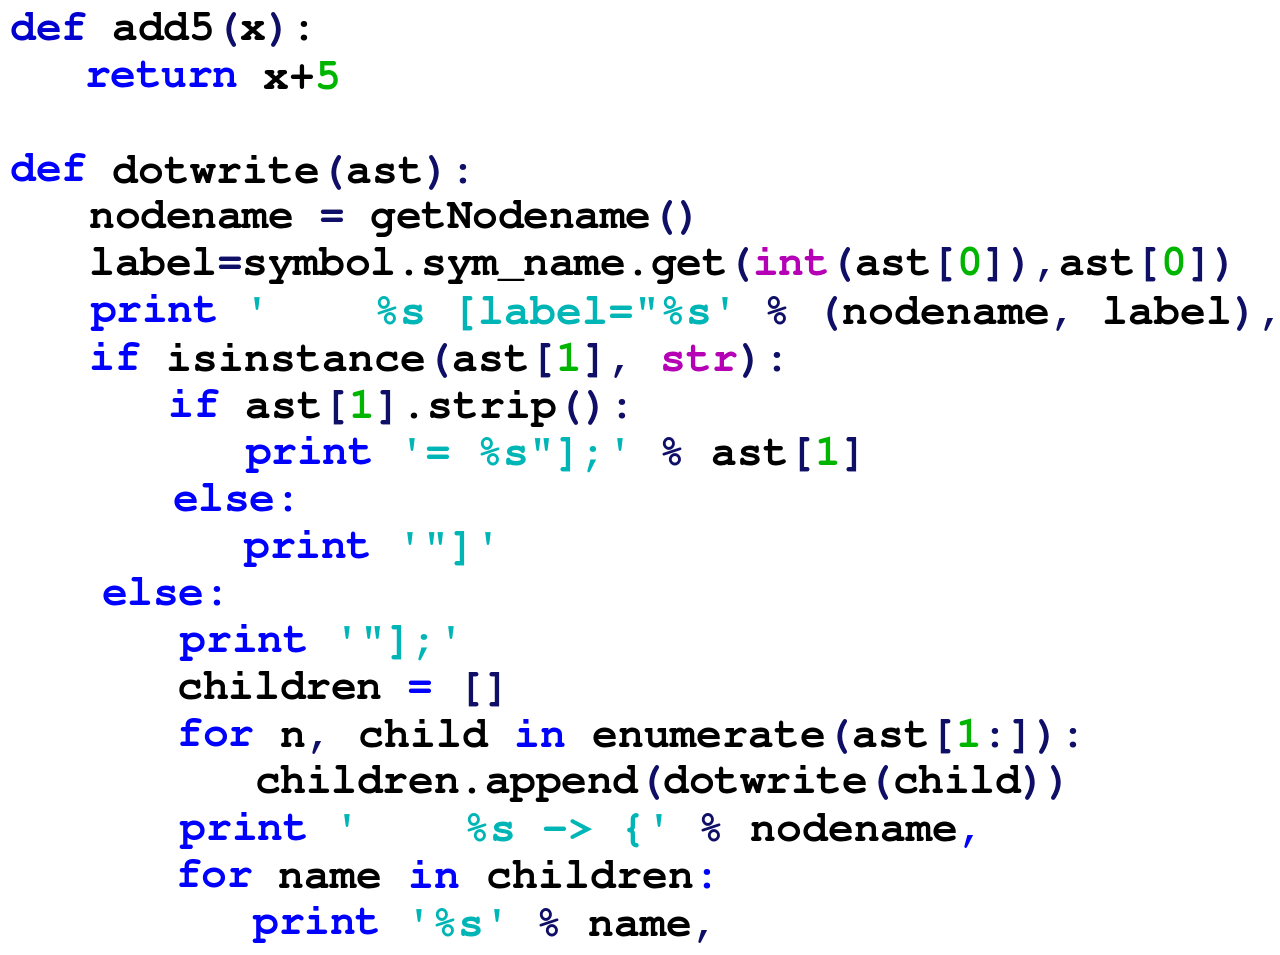
\includegraphics[width=0.7\textwidth]{img/pythonCode.png}
    %\caption{Before the Rename}
%    \label{fig:Python}
%  \end{figure}
%\end{frame}
%\begin{frame}{Related Work}
%  \begin{itemize}
%  \item {
%    First item.
%    \pause % The slide will pause after showing the first item
%  }
%  \item {
%    Second item.
%  }
  % You can also specify when the content should appear
  % by using <n->:
%  \item<3-> {
%    Third item.
%  }
%  \item<4-> {
%    Fourth item.
%  }
  % or you can use the \uncover command to reveal general
  % content (not just \items):
%  \item<5-> {
%    Fifth item. \uncover<6->{Extra text in the fifth item.}
%  }
%  \end{itemize}
%\end{frame}

\begin{frame}{Racket}
\begin{figure}[htbp]
  \centering
  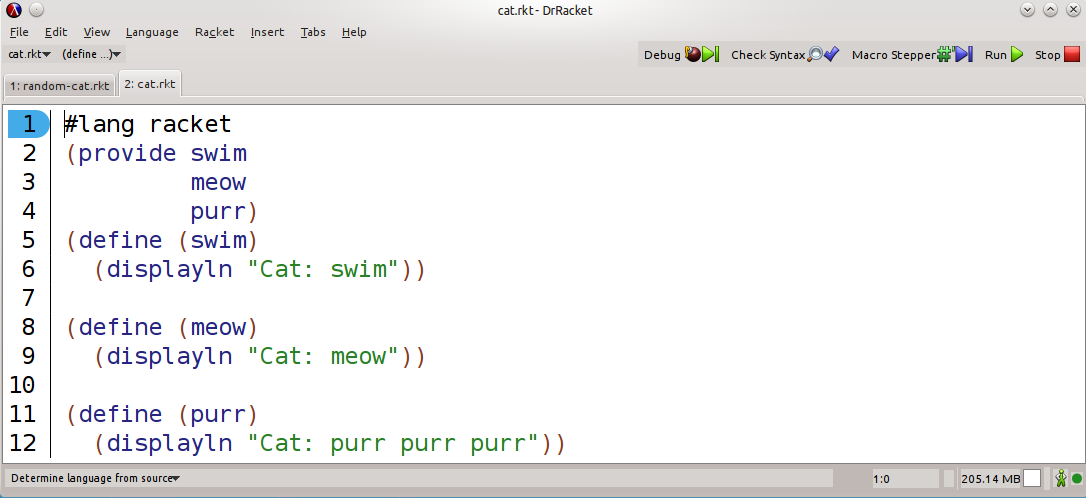
\includegraphics[width=0.7\textwidth]{img/cat-definition.png}
  %\caption{Before the Rename}
  \label{fig:renameBefore}
\end{figure}
\end{frame}
\begin{frame}{DrRacket's Rename}
\begin{figure}[htbp]
  \centering
  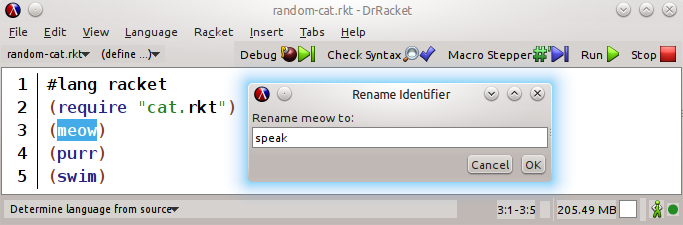
\includegraphics[width=0.7\textwidth]{img/renameV3-2.png}
  %\caption{Before the Rename}
  \label{fig:renameBefore}
\end{figure}

\begin{figure}[htbp]
  \centering
  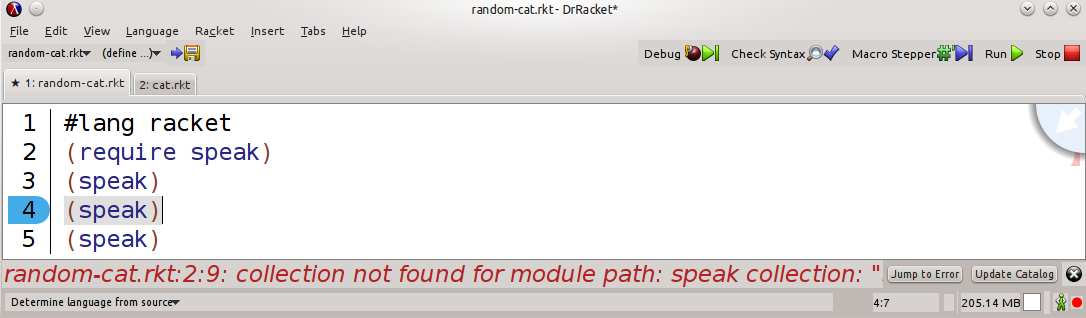
\includegraphics[width=0.7\textwidth]{img/rename-error.png}
  %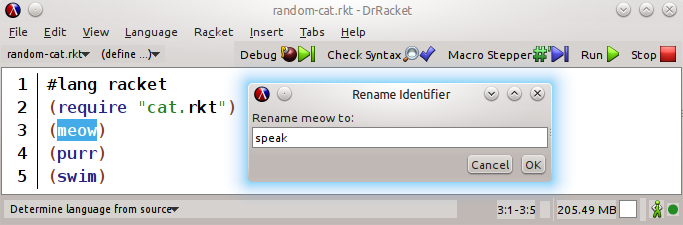
\includegraphics[width=0.7\textwidth]{img/renameV3-2.png}
  %\caption{Rename error on DrRacket}
  \label{fig:RacketBug}
\end{figure}
\end{frame}

\section{Solution}
%architecture image
\subsection{Architecture}
\begin{frame}{Architecture}
\begin{figure}[htbp]
  \centering
  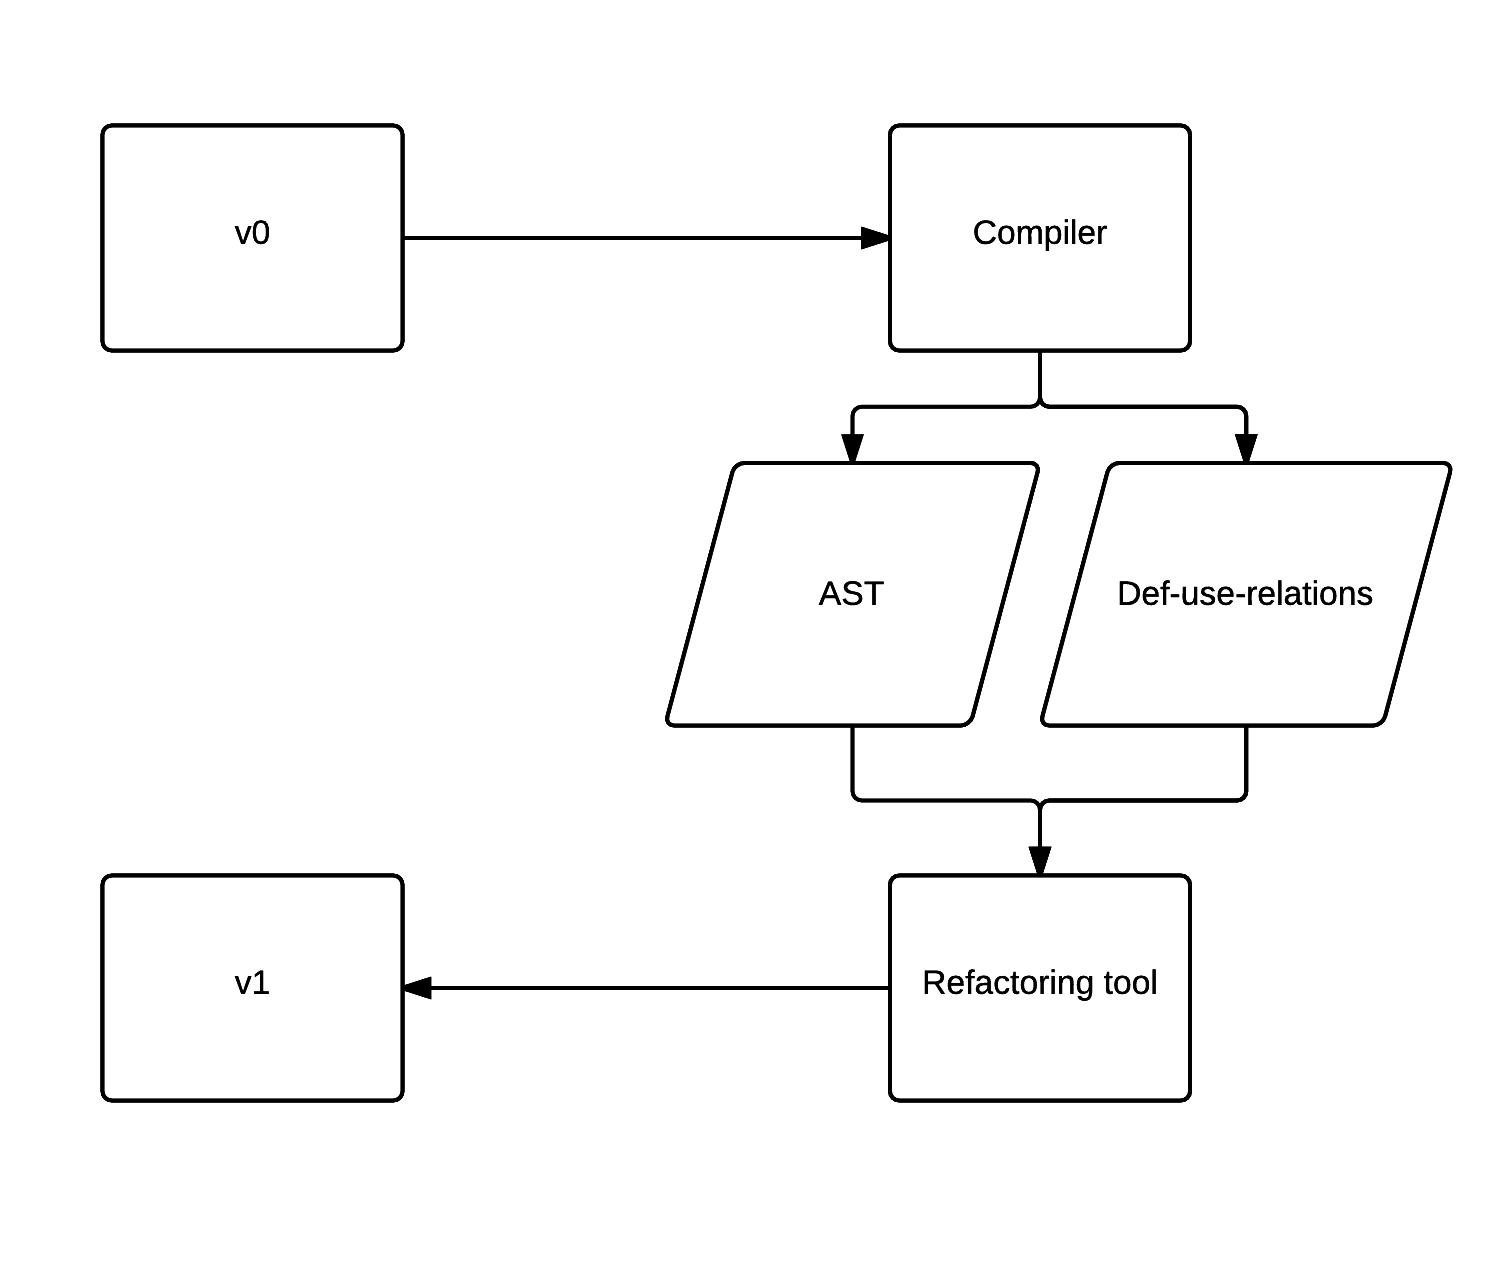
\includegraphics[width=0.65\textwidth]{img/arquitectura.png}
  %\caption{System Architecture}
  \label{fig:label}
\end{figure}
\end{frame}
\begin{frame}{Validation}
  \begin{itemize}
  \setlength\itemsep{2em}
  \item {
    Extract function
  }
  \item {
    Rename
  }
  \item {
    Add-Prefix
  }
  \end{itemize}
\end{frame}
\begin{frame}{Validation - Extract function}
%extract-function
\begin{figure}[htbp]
  \centering
  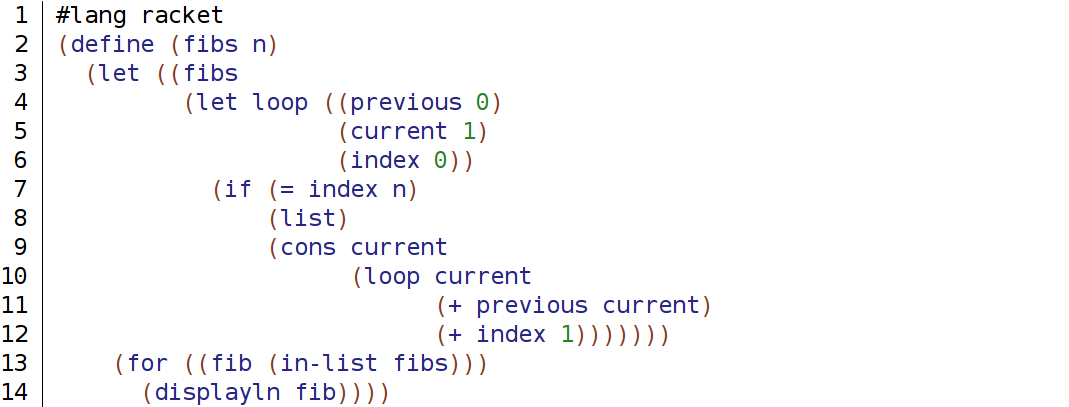
\includegraphics[width=0.7\textwidth]{img/fibonacci-1.png}
  %\caption{Rename error on DrRacket}
  \label{fig:fib-extract}
\end{figure}

\begin{figure}[htbp]
  \centering
  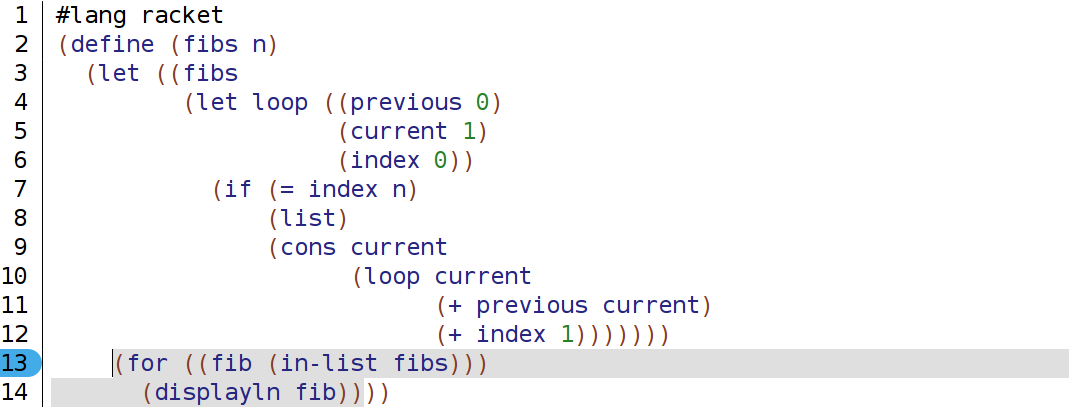
\includegraphics[width=0.7\textwidth]{img/fibonacci-select.png}
  %\caption{Rename error on DrRacket}
  \label{fig:fib-extract-one}
\end{figure}
\end{frame}
\begin{frame}{Validation - Extract function}
\begin{figure}[htbp]
  \centering
  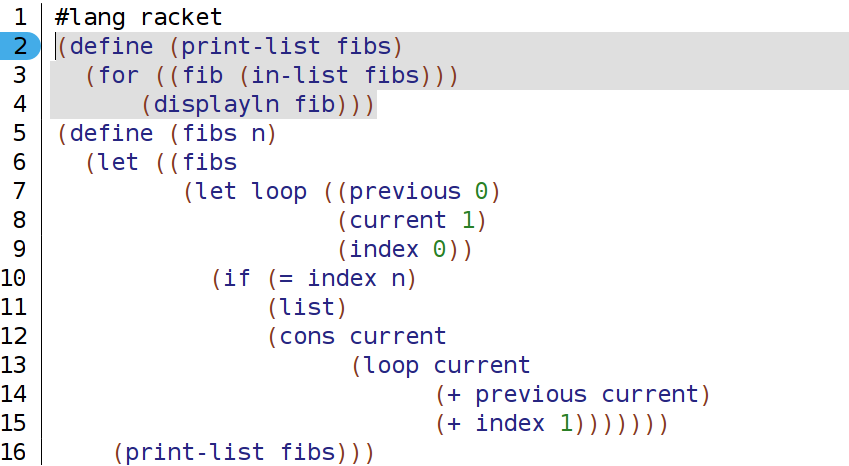
\includegraphics[width=0.7\textwidth]{img/fibonacci-After.png}
  %\caption{Rename error on DrRacket}
  \label{fig:fib-extract-two}
\end{figure}
\end{frame}
\begin{frame}{Validation - Rename}
%Rename
\begin{figure}[htbp]
  \centering
  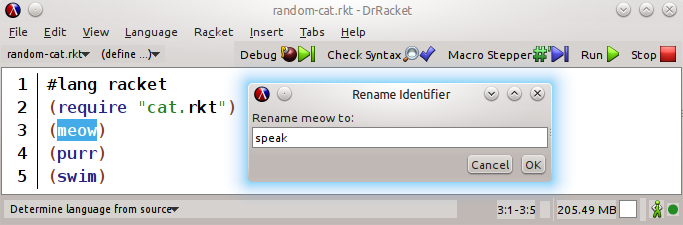
\includegraphics[width=0.7\textwidth]{img/renameV3-2.png}
  %\caption{Rename error on DrRacket}
  \label{fig:RenameCorrectBefore}
\end{figure}

\begin{figure}[htbp]
  \centering
  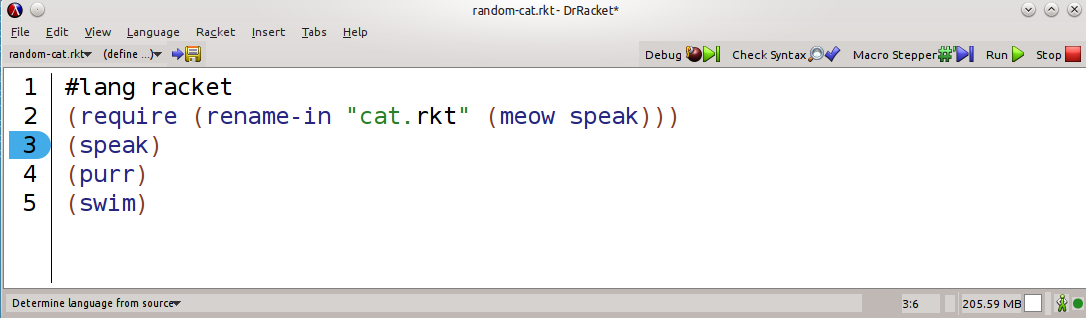
\includegraphics[width=0.7\textwidth]{img/renameV2-Correct-2.png}
  %\caption{Rename error on DrRacket}
  \label{fig:RenameCorrectAfter}
\end{figure}
\end{frame}
\begin{frame}{Validation - Add prefix}
%add-prefix
\begin{figure}[htbp]
  \centering
  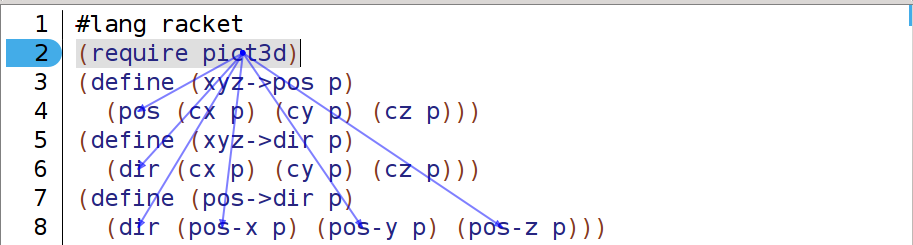
\includegraphics[width=0.7\textwidth]{img/add-prefixV2-1.png}
  %\caption{Rename error on DrRacket}
  \label{fig:AddPrefixBefore}
\end{figure}
\begin{figure}[htbp]
  \centering
  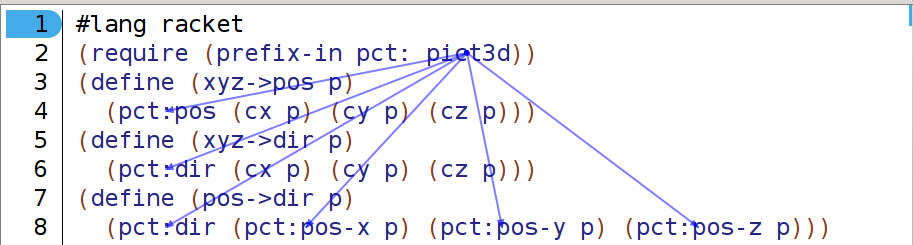
\includegraphics[width=0.7\textwidth]{img/add-prefixV2-3.png}
  %\caption{Rename error on DrRacket}
  \label{fig:AddPrefixAfter}
\end{figure}
\end{frame}
%\begin{frame}{Solution}
%\begin{block}{Block Title}
%You can also highlight sections of your presentation in a block, with it's own title
%\end{block}
%\begin{theorem}
%There are separate environments for theorems, examples, definitions and proofs.
%\end{theorem}
%\begin{example}
%Here is an example of an example block.
%\end{example}
%\end{frame}

\subsection{Evaluation}
\begin{frame}{Evaluation}

\begin{itemize}
  \setlength\itemsep{2em}
\item Refactoring Correctness
\item Usability and Simplicity
\end{itemize}
\end{frame}
%\section{Conclusion}
%\begin{frame}{test}
%\end{frame}
%\section*{this is another test}
%\begin{frame}{test2}
%\end{frame}
% Placing a * after \section means it will not show in the
% outline or table of contents.
%\section*{Summary}

%\begin{frame}{Summary}
%  \begin{itemize}
%  \item
%    There is a lack of refactoring tools adequate for inexperienced users
%  \item
%    The \alert{second main message} of your talk in one or two lines.
%  \item
%    Perhaps a \alert{third message}, but not more than that.
%  \end{itemize}

%  \begin{itemize}
%  \item
%    Outlook
%    \begin{itemize}
%    \item
%      Something you haven't solved.
%    \item
%      Something else you haven't solved.
%    \end{itemize}
%  \end{itemize}
%\end{frame}



% All of the following is optional and typically not needed.
\appendix
\section<presentation>*{\appendixname}
%\subsection<presentation>*{}
%\addtobeamertemplate{last page}{ 
\includegraphics[scale=0.1]{img/IST_A_RGB_POS3.png} }{} %por a imagem no canto superior esquerdo.
\begin{frame}
\begin{center}

{\Large Thank you!}
\\~\\
\leavevmode\\~\\
{\Huge Questions?}
\end{center}

\end{frame}

%\begin{frame}[allowframebreaks]
%  \frametitle<presentation>{For Further Reading}
%
%  \begin{thebibliography}{10}
%
%  \beamertemplatebookbibitems
%  % Start with overview books.
%
%  \bibitem{Author1990}
%    A.~Author.
%    \newblock {\em Handbook of Everything}.
%    \newblock Some Press, 1990.
%
%
%  \beamertemplatearticlebibitems
%  % Followed by interesting articles. Keep the list short.
%
%  \bibitem{Someone2000}
%    S.~Someone.
%    \newblock On this and that.
%    \newblock {\em Journal of This and That}, 2(1):50--100,
%    2000.
%  \end{thebibliography}
%\end{frame}

\end{document}
